\documentclass[tikz,border=2pt]{standalone}
\usepackage{amsmath}
\usepackage{tikz}

\begin{document}
% 1/2 + 1/4 + 1/8 + ... fills the unit square: the partial sums approach 1 and never exceed it.
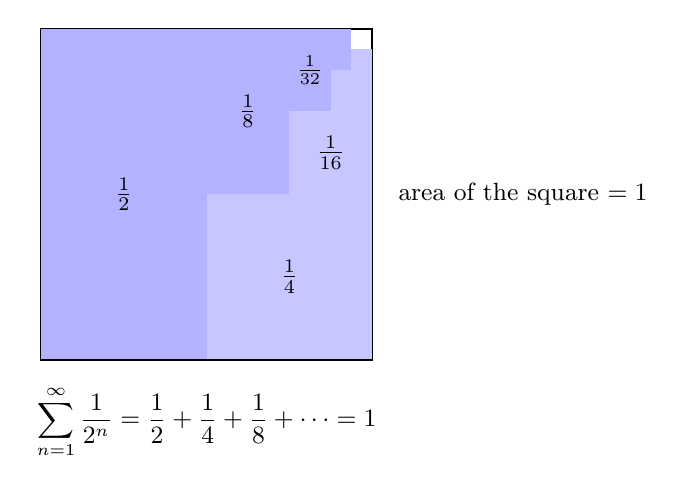
\begin{tikzpicture}[scale=4.2]
	\draw[thick] (0,0) rectangle (1,1);
	\fill[blue!30] (0,0) rectangle (0.5,1);      \node at (0.25,0.5) {$\tfrac12$};
	\fill[blue!22] (0.5,0) rectangle (1,0.5);    \node at (0.75,0.25) {$\tfrac14$};
	\fill[blue!30] (0.5,0.5) rectangle (0.75,1); \node at (0.625,0.75) {$\tfrac18$};
	\fill[blue!22] (0.75,0.5) rectangle (1,0.75);\node at (0.875,0.625) {$\tfrac1{16}$};
	\fill[blue!30] (0.75,0.75) rectangle (0.875,1); \node[font=\small] at (0.8125,0.875) {$\tfrac1{32}$};
	\fill[blue!22] (0.875,0.75) rectangle (1,0.875);
	\fill[blue!30] (0.875,0.875) rectangle (0.9375,1);
	\fill[blue!22] (0.9375,0.875) rectangle (1,0.9375);
	\node[anchor=north, font=\small] at (0.5,-0.05) {$\displaystyle\sum_{n=1}^{\infty}\frac1{2^n}=\frac12+\frac14+\frac18+\cdots=1$};
	\node[anchor=west, font=\small] at (1.05,0.5) {area of the square $=1$};
\end{tikzpicture}
\end{document}
